\documentclass{article}
\usepackage{amsmath}
\usepackage{graphicx}

\begin{document}

\title{COMP 5660 Fall 2024 Assignment 1a}
\author{Logan Bolton - ldb0046@auburn.edu}
\date{}

\maketitle

\section{Graphs}
\subsection{Stairstep Plots}
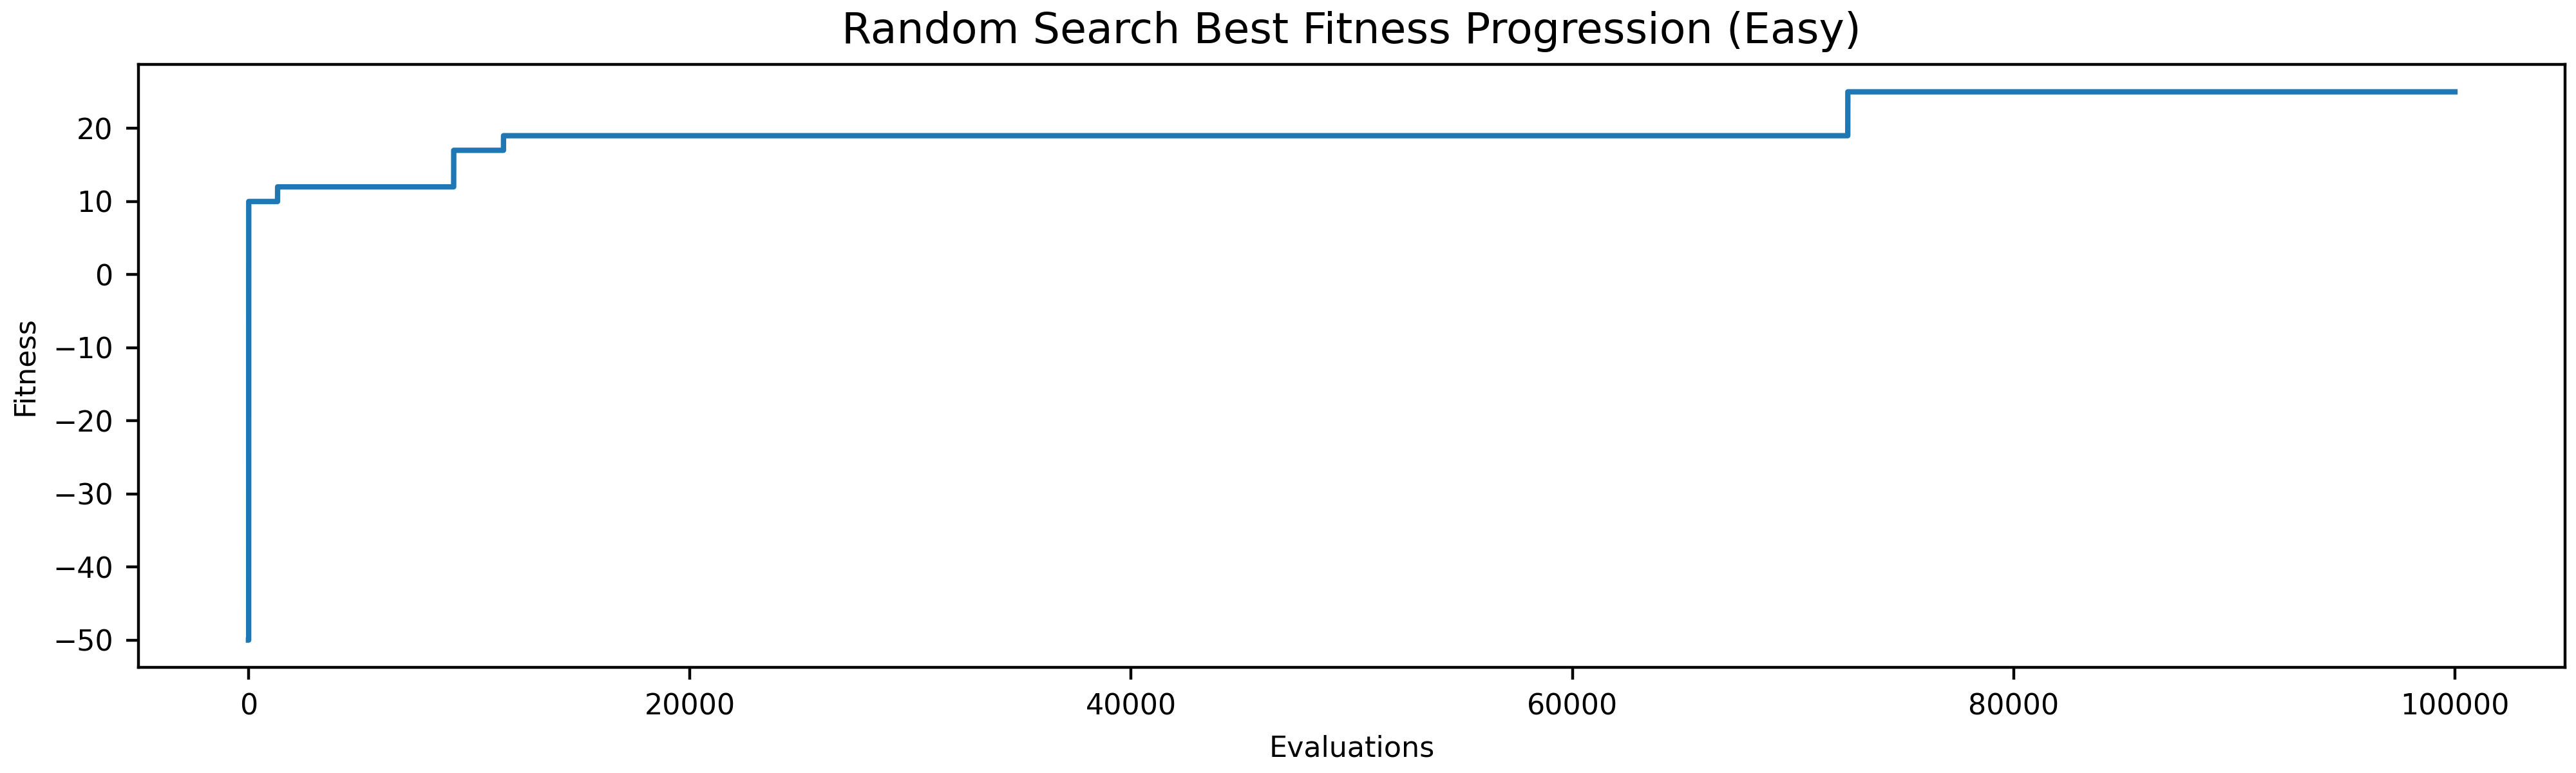
\includegraphics[width=\textwidth]{stairstep.png}
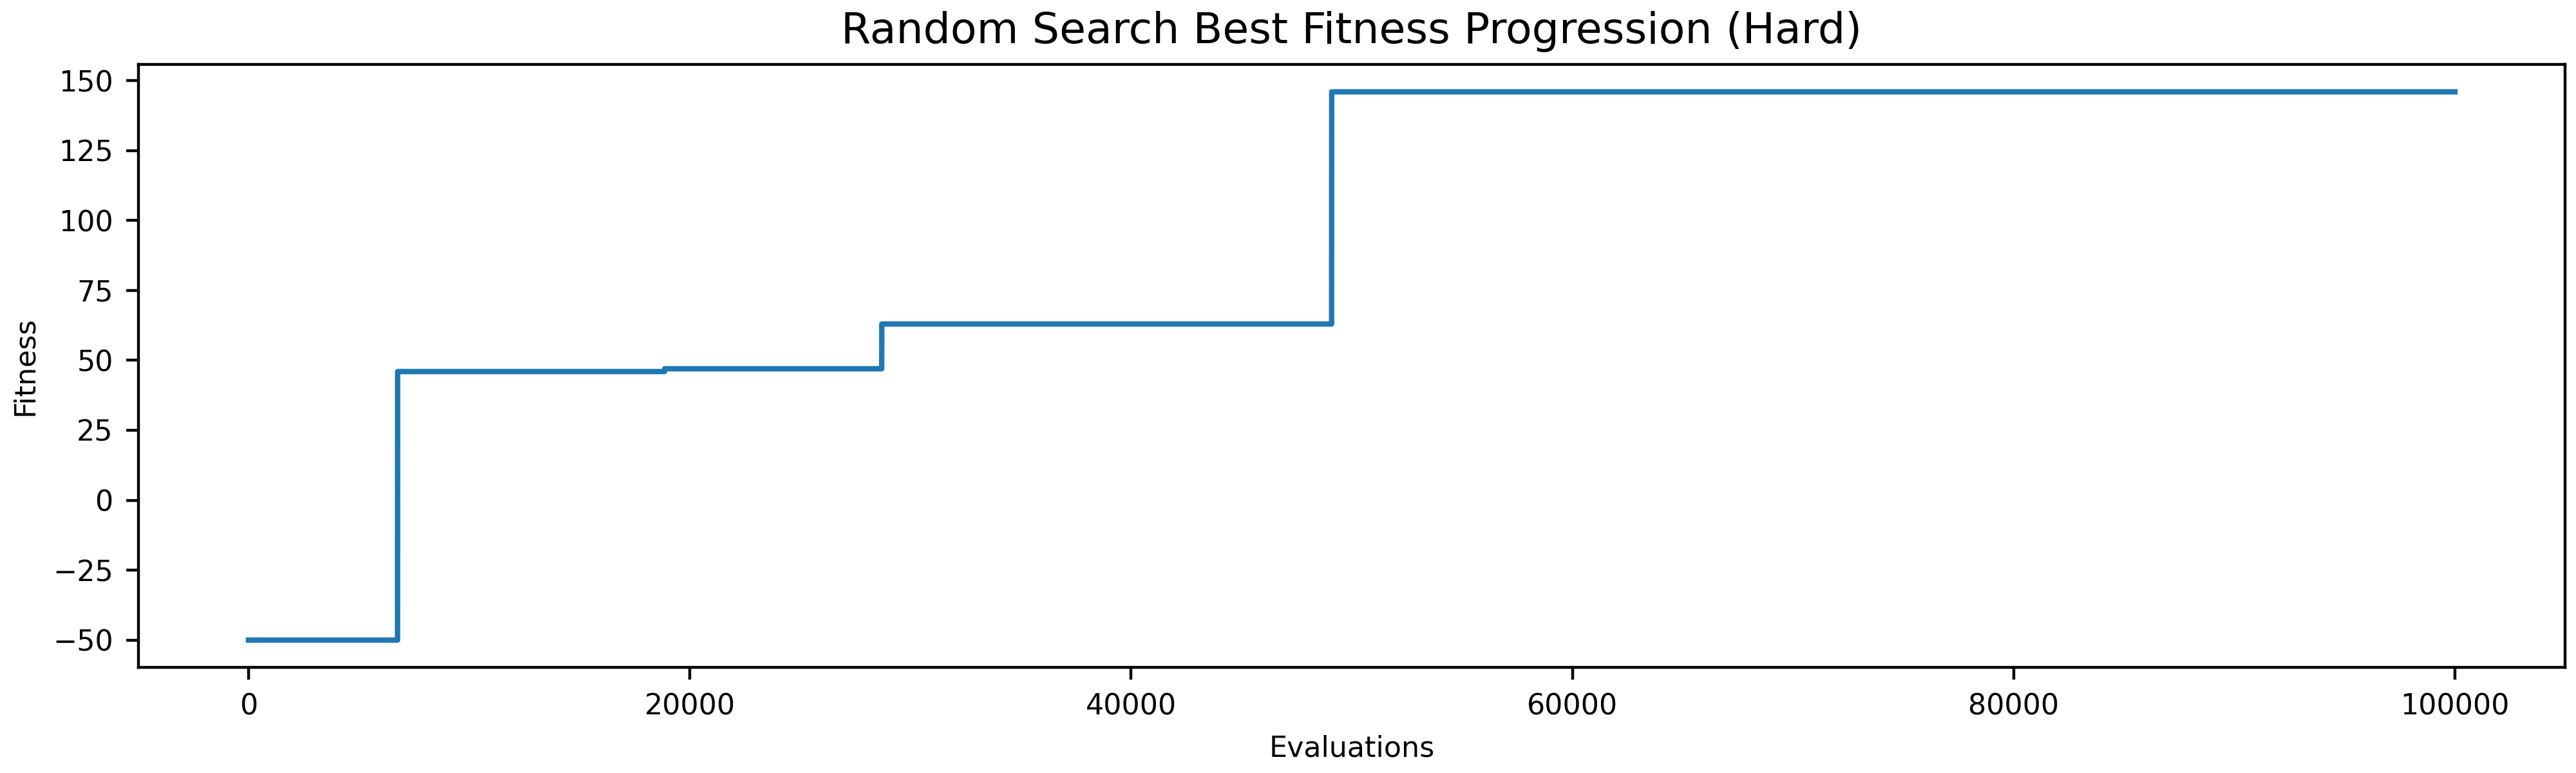
\includegraphics[width=\textwidth]{/Users/log/Github/stock1a-LoganBolton/data/1a/hard/stairstep.png}

\subsection{Histogram Plots}
\includegraphics[width=\textwidth]{/Users/log/Github/stock1a-LoganBolton/data/1a/easy/histogram.png}
\includegraphics[width=\textwidth]{/Users/log/Github/stock1a-LoganBolton/data/1a/hard/histogram.png}
\subsection{Best Solutions}

\begin{figure}[ht]
    \centering
    \includegraphics[width=\textwidth]{/Users/log/Github/stock1a-LoganBolton/data/1a/easy/best_solution.png}
    \caption{Best solution found after 30 runs of random search for the \textbf{easy} configuration.}
\end{figure}

\begin{figure}[ht]
    \centering
    \includegraphics[width=\textwidth]{/Users/log/Github/stock1a-LoganBolton/data/1a/hard/best_solution.png}
    \caption{Best solution found after 30 runs of random search for the \textbf{hard} configuration.}
\end{figure}

\pagebreak
\section{Statistical Analysis}
\subsection{Easy Mystery Data}


\begin{table}[ht]
\centering
\begin{tabular}{|c|c|c|}
\hline
\textbf{} & \textbf{Best Run - Random Search} & \textbf{Easy Mystery Data} \\
\hline
Mean Fitness & 21 & 37.46666666666667\\
\hline
Standard Deviation & 1.6815428055498771 & 1.0080138659874618\\

\hline
\# of samples & \multicolumn{2}{|c|}{30} \\
\hline
p-value & \multicolumn{2}{|c|}{5.029045257999176e-41} \\
\hline

$\alpha$-value & \multicolumn{2}{|c|}{0.05} \\\hline
\end{tabular}
\caption{Results of a T-test between the best runs of the random search and the runs of the easy mystery data set.}
\end{table}

Given that the p-value is much less than the $\alpha$-value, 
this means that the results between the random search and the easy mystery data
has a large statistical difference. Given that mean fitness of the mystery data is so much higher
and the standard deviation is also much lower, we can confidently conclude that the mystery
data is the best solution.
% \clearpage
\subsection{Hard Mystery Data}

\begin{table}[ht]
\centering
\begin{tabular}{|c|c|c|}
\hline
\textbf{} & \textbf{Best Run - Random Search} & \textbf{Hard Mystery Data} \\
\hline
Mean Fitness & 83.16666666666667 & 334.93333333333334\\
\hline
Standard Deviation & 16.70449729519142 & 8.325007334917897\\

\hline
\# of samples & \multicolumn{2}{|c|}{30} \\
\hline
p-value & \multicolumn{2}{|c|}{1.4028859047989313e-46} \\
\hline

$\alpha$-value & \multicolumn{2}{|c|}{0.05} \\\hline
\end{tabular}
\caption{Results of a T-test between the best runs of the random search and the runs of hard mystery data set.}
\end{table}

Given that the p-value is much less than the $\alpha$-value, 
this means that the results between the random search and the hard mystery data
has a large statistical difference. Given that mean fitness of the mystery data is so much higher
and the standard deviation is also much lower, we can confidently conclude that the mystery
data is the best solution.

\end{document}